\section{Multi-measurement Methods for Graph Diffusion Acceleration}
\label{sec: multiprox}

In the previous section, we discussed how HiGenDiff can reduce the number of edge probabilities to compute during graph generation and thus reduce time complexity, while preserving very strong generalization performance. However, the choice of employing diffusion models has a negative effect on scalability, as unlike most generative machines, they require $T$ inference steps to produce a sample instead of simple one-shot generation.

This part of the thesis will argue that it is possible to reduce the number of denoising steps required, while also preserving baseline performance. Multi-measurement sampling theory is the key knowledge we must apply to achieve those effects. The content presented in this section is published as~\cite{dadi_improving_2025} and is also discussed in~\cite{dadi_noisy_2025}.

\subsection{The One True Step}

As we have seen before, denoising diffusion models generate samples by first training a sequence of denoisers at various noise levels and cleverly chaining them to transform unstructured random noise into a sample from a target distribution~\cite{ho_denoising_2020, dhariwal_diffusion_2021}. 

The different noise levels, the methods in which the denoisers are chained, and the balancing of the loss for different noise levels all require careful tuning~\cite{karras_elucidating_2022}. So much so that one might ask why we must sample using different noise levels and not simply just one? Why is the annealing (i.e., the gradual decrease of noise) during the sampling stage necessary? 

The reason, as discussed in Section~\ref{sec:background_multiprox}, is to break down a difficult sampling problem into a sequence of unimodal sampling problems. Indeed, distributions of interest such as natural images are often multi-modal. The denoising diffusion framework breaks down this sampling task into a sequence of unimodal distributions that are easily approximated by Gaussians. 

In this work, we show that this sequence of simpler distributions need not be at different noise levels. To propose our framework that operates at a single noise level, we build on ideas from log-concave sampling.

In particular, we build on the work of~\cite{saremi_multimeasurement_2022} and earlier investigations in~\cite{jain_journey_2022}, which propose a single noise level generative framework. Their sampling process involves sampling from a distribution that is not log-concave. To mitigate this,~\cite{saremi_chain_2024} proposes a \emph{chain of log-concave} breakdowns of the task, but at the cost of requiring denoisers at several different noise scales. Moreover, their work merely guarantees that the distributions sampled in their framework are \emph{increasingly} log-concave. 

The following question remained unanswered:
\begin{center}
    \emph{Is there an entirely log-concave single-noise level generative framework?}
\end{center}

In this work, we first study the case when the unnormalized log-density is known to propose the MultiProx sampler. Then, we conduct experiments to show that our framework still yields good results when using a score function from data on real datasets. 

\subsection{Background}
\label{sec:background_multiprox}

In this preliminary section, we present the necessary background on the variance-preserving variant of Denoising Diffusion Probabilistic Models (DDPMs)~\cite{ho_denoising_2020}. Our goal is to characterize the motivation for \emph{time annealing} in diffusion models and question its necessity. 

\subsubsection{DDPMs and the motivation behind annealing}

Recall that, for a data distribution $\mathbf{X}_0 \sim p_0$ over $\mathbb{R}^F$, DDPMs first learn how to denoise by generating noisy versions of $p_0$ (i.e., the forward process). Concretely, noisy measurements $\mathbf{X}_t$, with density denoted $p_t$, of the target distribution are generated as  
\begin{equation}
\mathbf{X}_t = \alpha_t \mathbf{X}_0 +\beta_t Z_t,
\label{eq:noising}
\end{equation}
where $Z_t \sim N\of{\mathbf{0}, \mathbf{I}_F}$ is an independently sampled standard Gaussian; and $\mathbf{X}_0$ is a sample from the data distribution $p_0$. Given these noisy measurements, a network $g_t:\mathbb{R}^F\to\mathbb{R}^F$ is trained to denoise $\mathbf{X}_t$ by learning to predict the noise $Z_t$ given $\mathbf{X}_t$. This boils down to approximating the rescaled score of $\mathbf{X}_t$ given by $-\beta_t \nabla \log p_t$. With simple algebra, we can show that the network is merely a reparametrized approximation to the conditional expectation of $\mathbf{X}_0|\mathbf{X}_t$. In other words, we can show that
\begin{equation}
\label{eq:reparam}
\frac{1}{\alpha_t}\off{X_t - \beta_t g_t\of{\mathbf{X}_t}} = \mathbb{E}\off{\mathbf{X}_0|\mathbf{X}_t}.
\end{equation}
Once the network is trained, diffusion models use this network to progressively denoise a standard Gaussian to generate new samples. The network has learned to compute conditional expectations, and the goal of the denoising process is to exploit these conditional expectations to output a new sample. 

If $T$ is the largest amount of noise added during training, the denoising process starts from an approximation $\tilde{\mathbf{X}}_T$ of $\mathbf{X}_T$, which is sampled from a standard Gaussian $N\of{\mathbf{0}, \mathbf{I}_F}$. The closer the distribution of $\tilde{\mathbf{X}}_T$ is to $p_T$, the better: the quality of the Gaussian initialization improves as $T$ increases since the larger $T$ is, the closer $p_T$ is to $N\of{\mathbf{0}, \mathbf{I}_F}$. After the initialization, the denoising is achieved by simulating the reverse process. A single step of the latter yields the following Gaussian approximation, 
\begin{equation}
\label{eq:revdiff}
    \mathbf{X}_0|\mathbf{X}_T \approx \mathbb{E}\off{\mathbf{X}_0|\mathbf{X}_T} + \sigma_T Z,
\end{equation}
where $Z \sim N\of{\mathbf{0}, \mathbf{I}_F}$. Unfortunately, this single-step estimation of $\mathbf{X}_0$ from $\mathbf{X}_T$ becomes increasingly poor as $T$ becomes large. This large discrepancy between $\mathbf{X}_0|\mathbf{X}_T$ and its Gaussian approximation $N\of{\mathbb{E}\off{\mathbf{X}_0|\mathbf{X}_T}, \sigma_T \mathbf{I}_F}$ is the \emph{central motivation for time-annealing}. One-step denoising does not work because $\mathbf{X}_0|\mathbf{X}_T$ is too multi-modal. Indeed, \emph{multi-modal distributions are not well approximated by their expectation}, so we must progressively denoise in smaller steps where multi-modality is not an issue and each individual step is well-approximated by a Gaussian distribution. 

To restate the trade-off: the one-step Gaussian approximation is increasingly worsened by large choices of $T$, yet we must choose $T$ to be large in order for the initialization at $\hat{\mathbf{X}}_T$ to be valid. Time annealing is precisely the design choice that allows diffusion models to balance these competing trade-offs. For any large $T$, we can define a discretization sequence $0 = t_0 < t_1 < \dots < t_N = T$ so that the Gaussian approximation $
\mathbf{X}_{t_{i-1}}|\mathbf{X}_{t_{i}} \approx \mathbb{E}\off{\mathbf{X}_{t_{i-1}}|\mathbf{X}_{t_{i}}} + \sigma_{t_{i-1}} Z_{t_{i-1}},$
where $Z_{t_{i-1}} \sim N\of{\mathbf{0}, \mathbf{I}_F}$ is valid. 

These Gaussian approximations using the conditional expectation correspond precisely to the exponential integration scheme with $N$ discretization points applied to~\ref{eq:revdiff}. This is the reason why annealing is necessary: it breaks down the difficult multi-modal sampling step of going from $\mathbf{X}_T$ to $\mathbf{X}_0$ into a sequence of uni-modal sampling problems $\mathbf{X}_{t_{i-1}}|\mathbf{X}_{t_i}$. 

Diffusion models are a sequence of Gaussian approximations, and time annealing is what makes these Gaussian approximations valid by defining a sequence of steps over which Gaussian approximations using the learned conditional expectations are appropriate. This comes at a cost: a series of conditional expectations $\mathbb{E}\off{\mathbf{X}_{t_{i-1}}|\mathbf{X}_{t_{i}}}$ must be approximated, which requires denoisers at different noise scales.

\subsubsection{The disadvantages of time annealing}

Having expounded on the motivation for time-annealing, we now argue that time-annealing comes with critical drawbacks.

First, annealing is taxing to the denoising network. In practice, the most successful denoising networks are built on the ADM networks of~\cite{dhariwal_diffusion_2021}, which have been carefully improved in~\cite{karras_analyzing_2024}. There, a single network is trained to denoise samples at varying noise scales, where a separate component informs the network of the noise level.

The task of denoising varies greatly at different noise scales. At high-noise levels, the denoiser must learn how to introduce low-frequency elements in the samples; at low-noise levels, it must act solely on the high frequencies to introduce detail. Performing both these tasks using the same network requires careful balancing of the training loss. Indeed, as observed in~\cite{karras_analyzing_2024}, a multi-task training approach is adopted to stabilize training. Denoising different noise levels can be so radically different that recent work~\cite{balaji_ediff-i_2022} trains an ensemble of denoisers that separately focus on the high-noise and low-noise stages. In addition to the architectural difficulties, time annealing also introduces tuning difficulties: the training noise schedule was observed to be highly sensitive to the output resolution in~\cite{chen_importance_2023}. 
%Finally, taking inspiration from~\cite{rissanen_generative_2022, dieleman_diffusion_2024}, we perform a frequency analysis on intermediate images generated during the denoising process of a standard diffusion model, EDM~\cite{karras_elucidating_2022}.
Finally, time-annealing schedules, despite requiring architectural modifications and meticulous tuning, are observed to result in a significant portion of the denoising process adding minimal structural detail to the samples. The spectrum remains flat, akin to white noise, for a substantial part of the process.

In summary, while time annealing is a pivotal component as discussed earlier in this section, it places a considerable demand on the design of denoising architectures and necessitates precise tuning that is both resolution and dataset-dependent. Yet, a significant part of this process is spent without contributing any meaningful structure to the samples. 

In what follows, we will introduce an alternative approach to decomposing the sampling task. This method does not require a time-embedding sub-network and alleviates the tuning burden by reducing the number of variables involved, offering a more streamlined and efficient framework.

\subsection{Related work}

\paragraph{Diffusion Monte Carlo} Our work builds on previous schemes that mix ideas from log-concave sampling and denoising diffusions.
\cite{huang_reverse_2024} first introduces the idea of inner Langevin loops for sampling from potentials and provides a theoretical analysis. Similar ideas also appear in~\cite{mcdonald_proposal_2022} and~\cite{vargas_denoising_2023}, which incorporate score estimation for diffusive sampling, as do~\cite{akhound-sadegh_iterated_2024}.~\cite{chen_diffusive_2024} proposes DiGs, which corresponds exactly to the proximal sampler of~\cite{shen_composite_2020} made practical with MALA as an approximation. They circumvent the difficulty of sampling from high-noise levels by initializing in a \enquote{clever way}, which, unlike our proposal, is only a heuristic.~\cite{he_zeroth-order_2024} suggests a zeroth-order method to improve over the proximal sampler.~\cite{phillips_particle_2024} also proposes a sequential Monte Carlo scheme based on diffusions. The work of~\cite{chehab_practical_2024} reviews all recent tempering schemes. Crucially, the fundamental difficulty of the \emph{duality of log-concavity} which underlies sampling tasks is detailed in~\cite{grenioux_stochastic_2024}. It is this difficulty that our scheme addresses.

\paragraph{Multi-measurement process} Using multiple correlated measurements appears in~\cite{saremi_multimeasurement_2022} and~\cite{saremi_chain_2024}. More generally, multi-measurements correspond to linear observation as defined in~\cite{montanari_posterior_2024} or posterior sampling in linear regression with fixed design.

\subsection{The MultiProx samplers}
In section~\ref{sec:appendix_gibbs} of the appendix, we theoretically show how a technique called Gibbs multimeasurement is an entirely log-concave single-noise-level sampling framework. Each individual Gibbs sampling step is also computationally tractable, and each sampling step in Algorithm~\ref{alg:pipeline} can be implemented exactly. We derive from this result an implementation of our framework we call the MultiProx sampler, as Algorithm~\ref{alg:multiprox}.

\begin{algorithm}[H]
    \caption{The MultiProx sampler}
    \label{alg:multiprox}
    \begin{algorithmic}
        \STATE{\textbf{input} number of stages $n$, Gibbs ensemble size $m$, sampling frequency $p<m$, fixed noise level $t<T$, diffusion model generators $\offf{g_u}_{u=1}^{T}$}
        \STATE{$\hat{\mathbf{Y}}_1, \dots, \hat{\mathbf{Y}}_m \sim N\of{\mathbf{0},\mathbf{I}_{m F}}$}
        \FOR{$i \gets 1$ to $n$}
        \FOR{$j \gets 1$ to $m$}
        \STATE{$\hat{\mathbf{X}}_j\gets\frac{1}{m}\sum_{k=1}^{m}{\hat{\mathbf{Y}}_k}$}
        \STATE{$\hat{\mathbf{X}}_j \gets g_t\of{\hat{\mathbf{X}}_j}$}
        \IF{$p \mid j$}
        \STATE{\textbf{yield} $\hat{\mathbf{X}}_j$}
        \ENDIF
        \STATE{$\hat{\mathbf{Y}}_j \gets \hat{\mathbf{X}}_j$}
        \ENDFOR
        \ENDFOR
    \end{algorithmic}
\end{algorithm}

Figure~\ref{fig:multiprox} summarizes the MultiProx algorithm and its theoretical properties. Namely, note how with specific conditions on the number of multimeasurements $m$ and the fixed noise level $t$, Gibbs sampling provides us with a fully log-concave single-noise level denoising diffusion sampling framework. While the Gibbs sampling itself can easily be implemented with simple averaging and replacement of each multimeasurement one by one.

\begin{figure}[H]
    \centering
    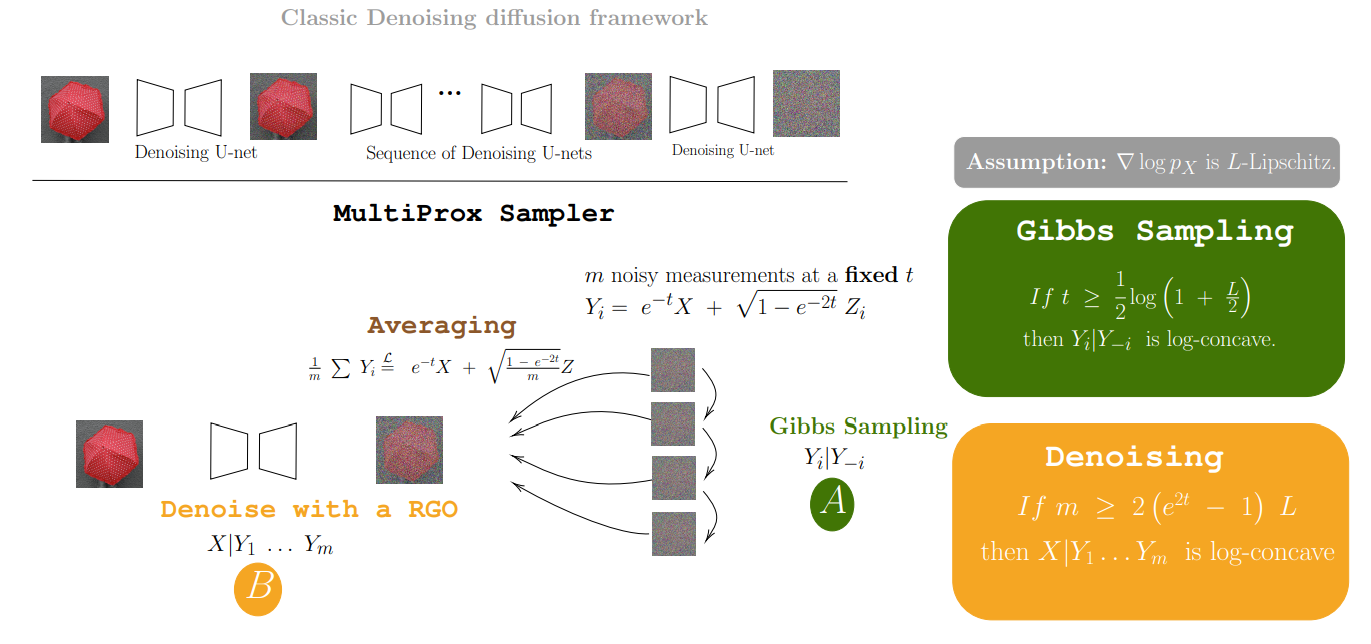
\includegraphics[width=\textwidth]{figures/multiprox/diagram.png}
    \caption[MultiProx diagram.]{Diagram of the operation of the MultiProx algorithm and the associated theoretical results, in comparison to the annealing baseline.}
    \label{fig:multiprox}
\end{figure}

Nevertheless, we did question the possibility that the assumption of Gaussian latent noise being appropriate for all non-modal distributions is invalid. In such a case, we hypothesize that sampling from a single noise level could be insufficient. We thus also consider allowing a few annealing steps to a second lower noise level $t' \leq t$ before outputting a sample and using it for Gibbs sampling. We refer to this modified sampling algorithm as MultiProxAn, whose pseudocode is given in Algorithm~\ref{alg:multiproxan}.

\begin{algorithm}%[H]
    \caption{The MultiProxAn sampler}
    \label{alg:multiproxan}
    \begin{algorithmic}
        \STATE{\textbf{input} number of stages $n$, Gibbs ensemble size $m$, sampling frequency $p<m$, fixed noise levels $t' \leq t<T$, diffusion model generators $\offf{g_u}_{u=1}^{T}$}
        \STATE{$\hat{\mathbf{Y}}_1, \dots, \hat{\mathbf{Y}}_m \sim N\of{\mathbf{0},\mathbf{I}_{m F}}$}
        \FOR{$i \gets 1$ to $n$}
        \FOR{$j \gets 1$ to $m$}
        \STATE{$\hat{\mathbf{X}}_j\gets\frac{1}{m}\sum_{k=1}^{m}{\hat{\mathbf{Y}}_k}$}
        \STATE{$\hat{\mathbf{X}}_j \gets \textcolor{blue}{\of{g_{t} \circ \dots \circ g_{t'}}}\of{\hat{\mathbf{X}}_j}$}
        \IF{$p \mid j$}
        \STATE{\textbf{yield} $\hat{\mathbf{X}}_j$}
        \ENDIF
        \STATE{$\hat{\mathbf{Y}}_j \gets \hat{\mathbf{X}}_j$}
        \ENDFOR
        \ENDFOR
    \end{algorithmic}
\end{algorithm}

\subsection{Experiments}

In this section, we present the results of a series of experiments conducted with MultiProx to confirm its effectiveness at sampling from multimodal distributions.

For most cases of interest, the log-density is not available and needs to be learnt from samples. In this case, exact Gibbs sampling techniques become too expensive to execute. For this reason alone, in the MultiProx pseudocode and in implementation, we approximate the true Restricted Gaussian Oracle (RGO) with the generator networks. Importantly, note that we do not retrain the diffusion models; we simply replace the annealing sampling strategy employed during evaluation with our own.

\subsubsection{Learnt score functions for images}
Figure~\ref{fig:multiprox_images} displays Gibbs chains of samples, obtained using MultiProx, from 3 image datasets: CIFAR10~\cite{krizhevsky_learning_2009}, AFHQ~\cite{choi_stargan_2020}, and FFHQ 64x64~\cite{karras_style-based_2019}. We observe how, after a few \enquote{warm-up} iterations, the chains smoothly interpolate between the complicated image modes.
\begin{figure}[H]
    \centering
    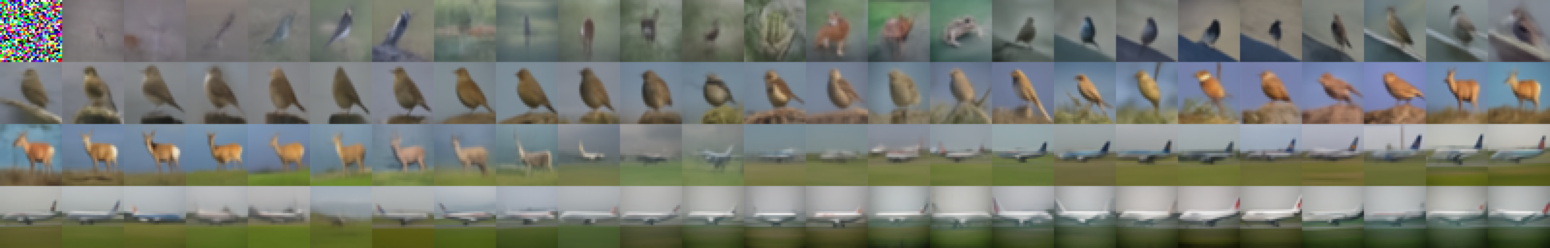
\includegraphics[width=0.49\linewidth]{figures/multiprox/cifar10.png}
    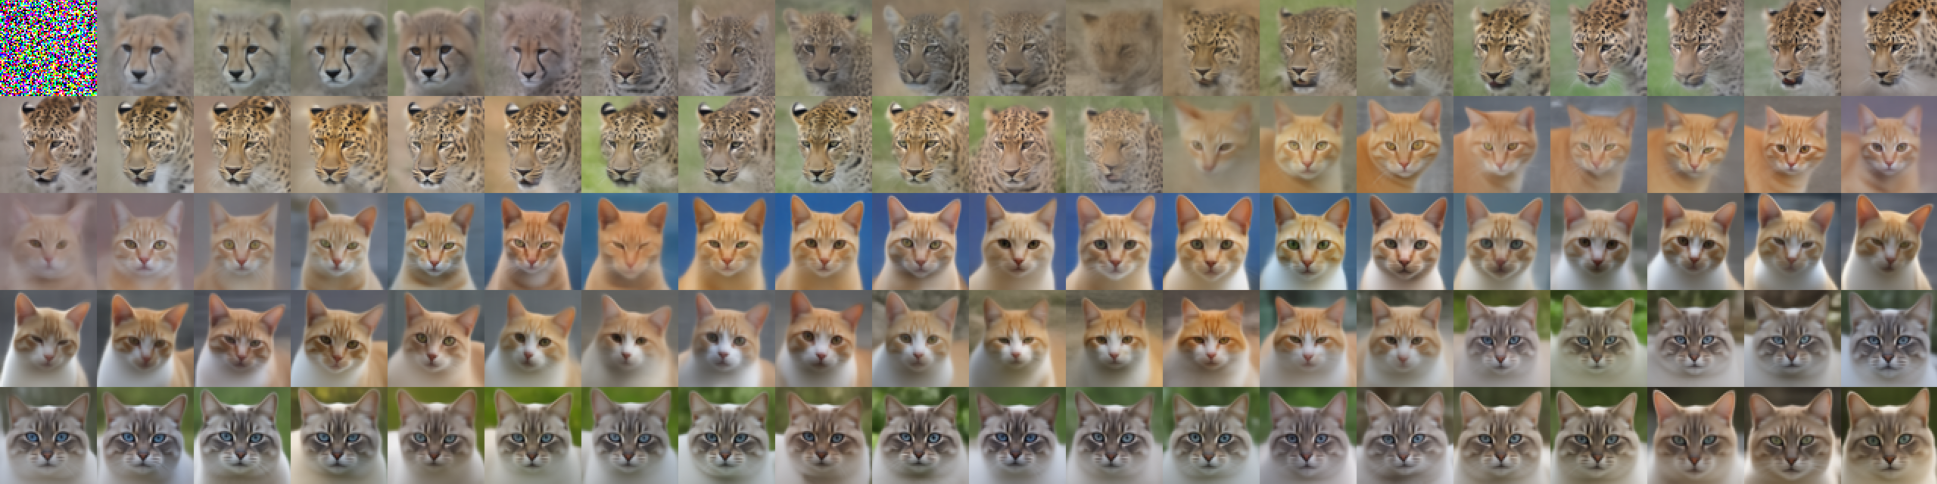
\includegraphics[width=0.49\linewidth]{figures/multiprox/afhq.png}
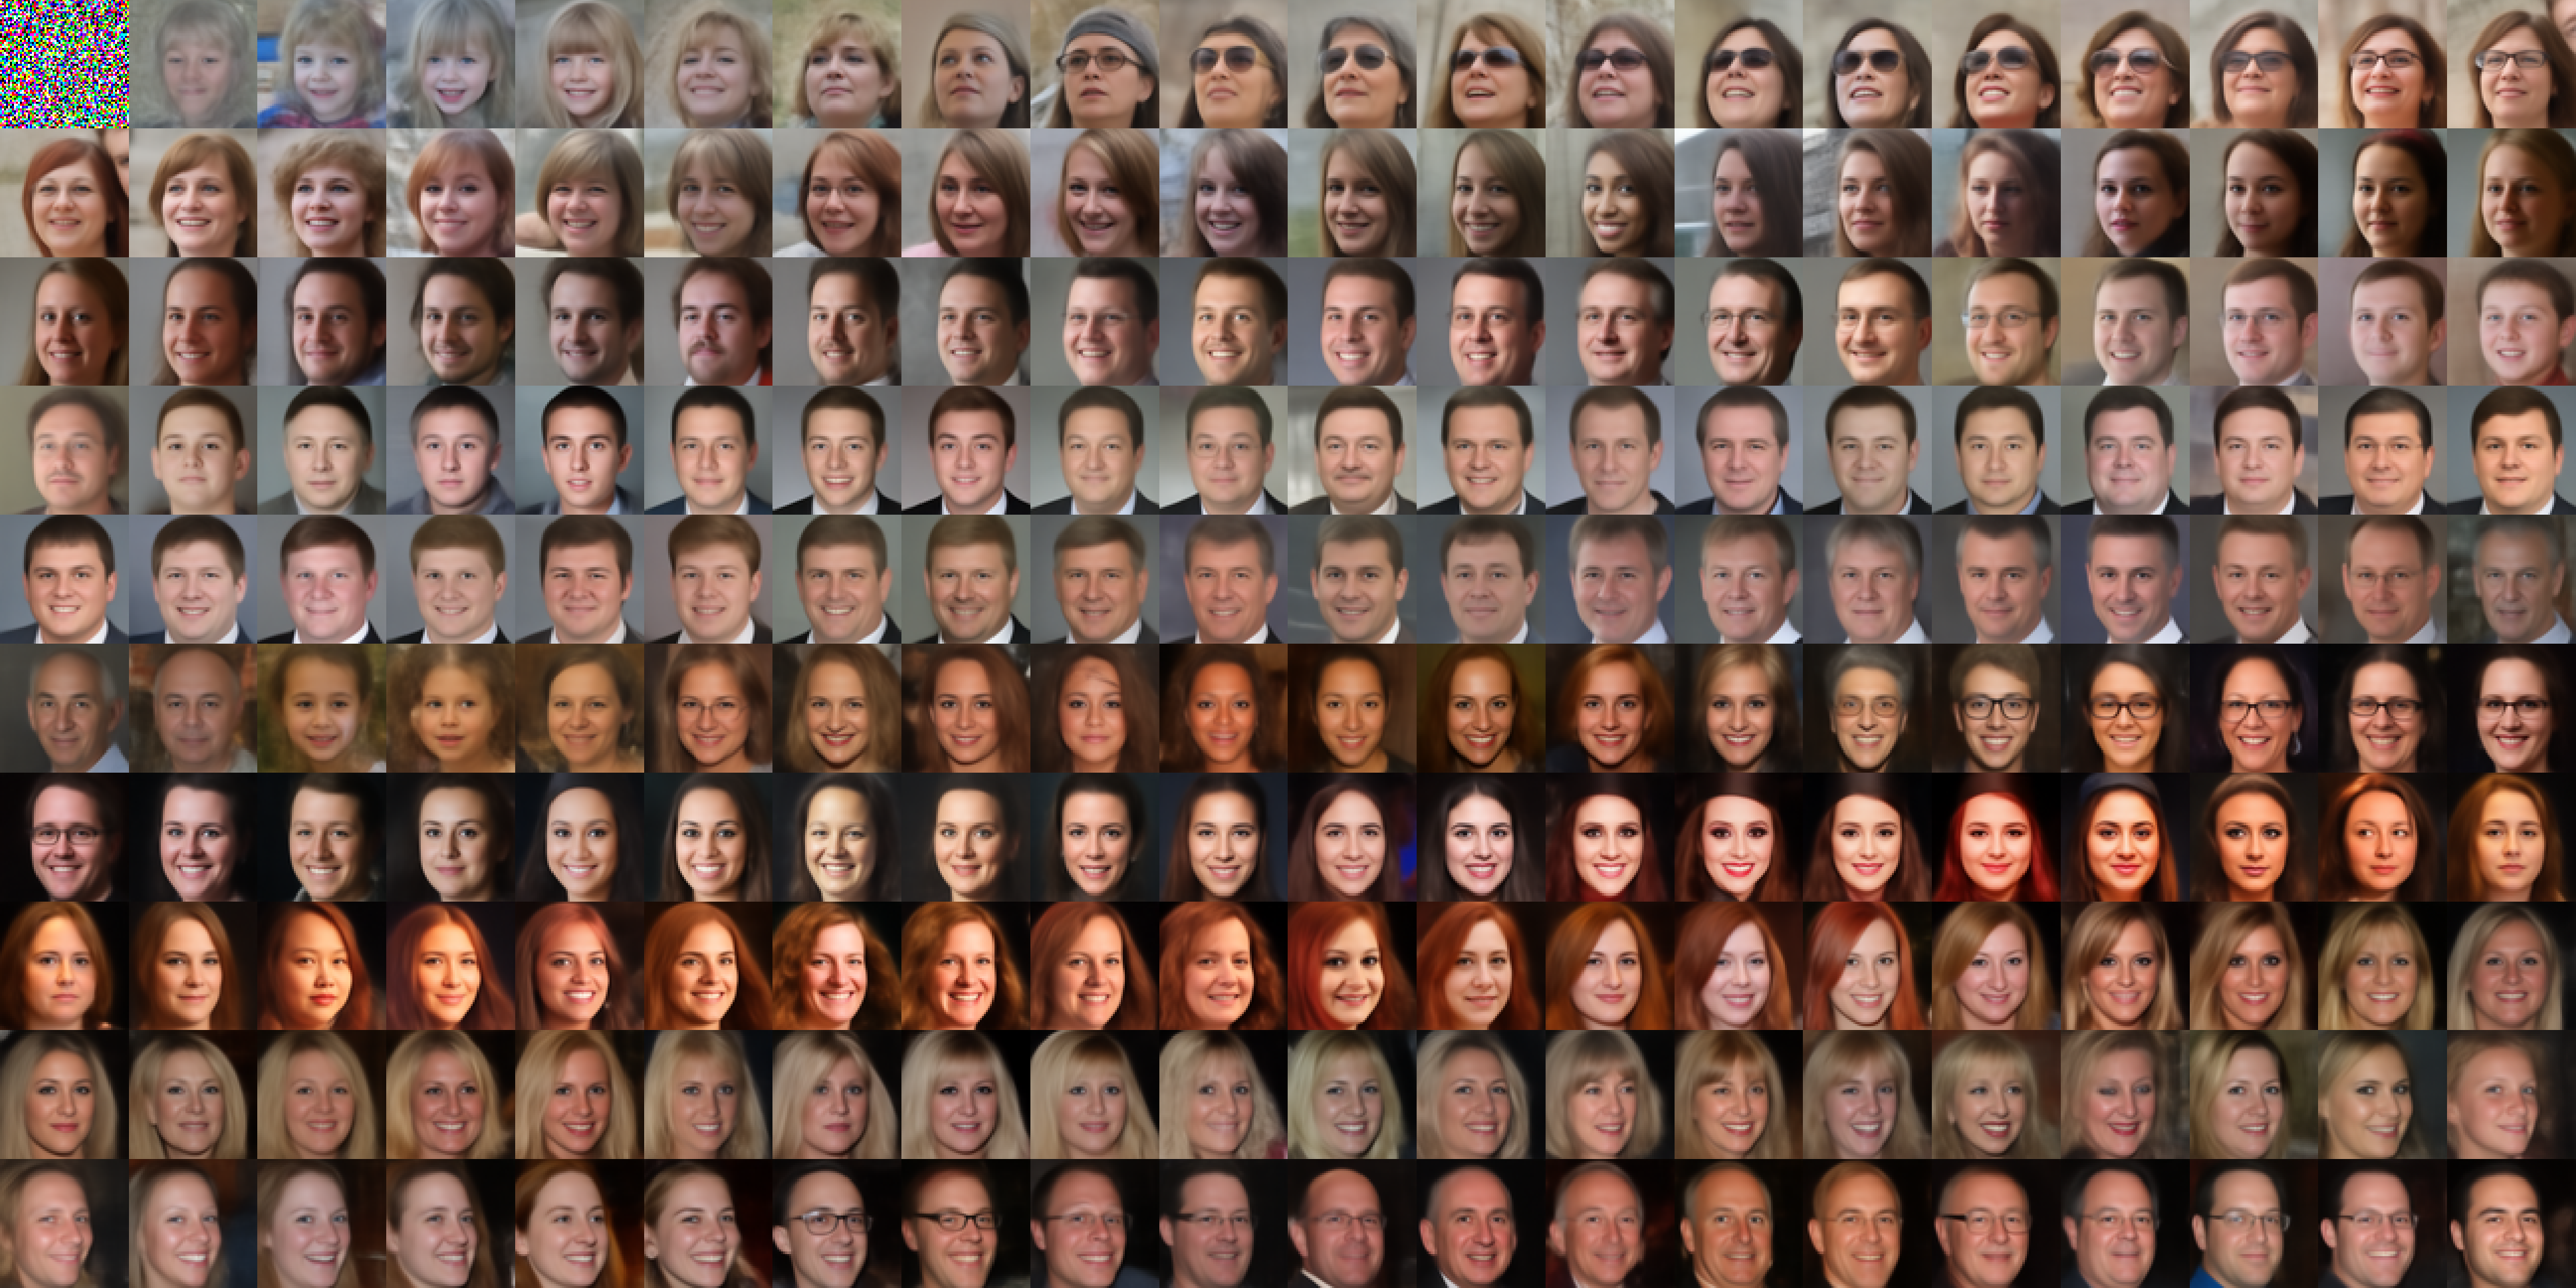
\includegraphics[width=0.75\linewidth]{figures/multiprox/ffhq.png}
    \caption{A single MultiProx chain of CIFAR10, AFHQ and FFHQ 64x64.}
    \label{fig:multiprox_images}
\end{figure} 

\subsubsection{Graphs}
In any case, the main experimental results that are relevant for this thesis work are those on discrete distributions. Modeling and sampling from discrete distributions such as graphs is a more complicated generative learning task. 

We thus focused on evaluating our sampling technique on two classical graph distribution learning tasks: learning to generate novel small molecular structures using the QM9 dataset of 9-node graphs with 4 atom (node) types and 5 bond (edge) types~\cite{ruddigkeit_enumeration_2012, ramakrishnan_quantum_2014}, and Community20, a toy dataset of 100 2-block SBM-sampled random graphs. Evaluation metrics for molecules include measuring the sampling rates of valid, unique, and novel molecular structures. For the simpler Community20 dataset lacking graph interpretation, one can perform Maximum Mean Discrepancy (MMD) statistical tests for the difference between sampled and true distributions of various classical graph features as before~\cite{gretton_kernel_2012, liao_efficient_2019}.

Graph diffusion model experiments differ from standard practice in that the noise process and denoising model act potentially on both continuous and discrete features, where discrete features are sampled through denoising the per-class log-probability and a final argmax over all logits to sample a graph node or edge type. DiGress~\cite{vignac_digress_2022}, the state-of-the-art model that we re-evaluated with MultiProx, also introduced the discrete noise process with a categorical instead of a Gaussian distribution; however, we focused on the authors' ConGress version with Gaussian continuous-space noising for consistency with other experiments. Figure~\ref{fig:multiprox_qm9} visualizes the molecule graphs in an example sampled Gibbs chain. Refer to Appendix~\ref{sec:appendix_multiprox_experiments} for our results on the Community20 dataset. 

\begin{figure}[H]
    \centering
    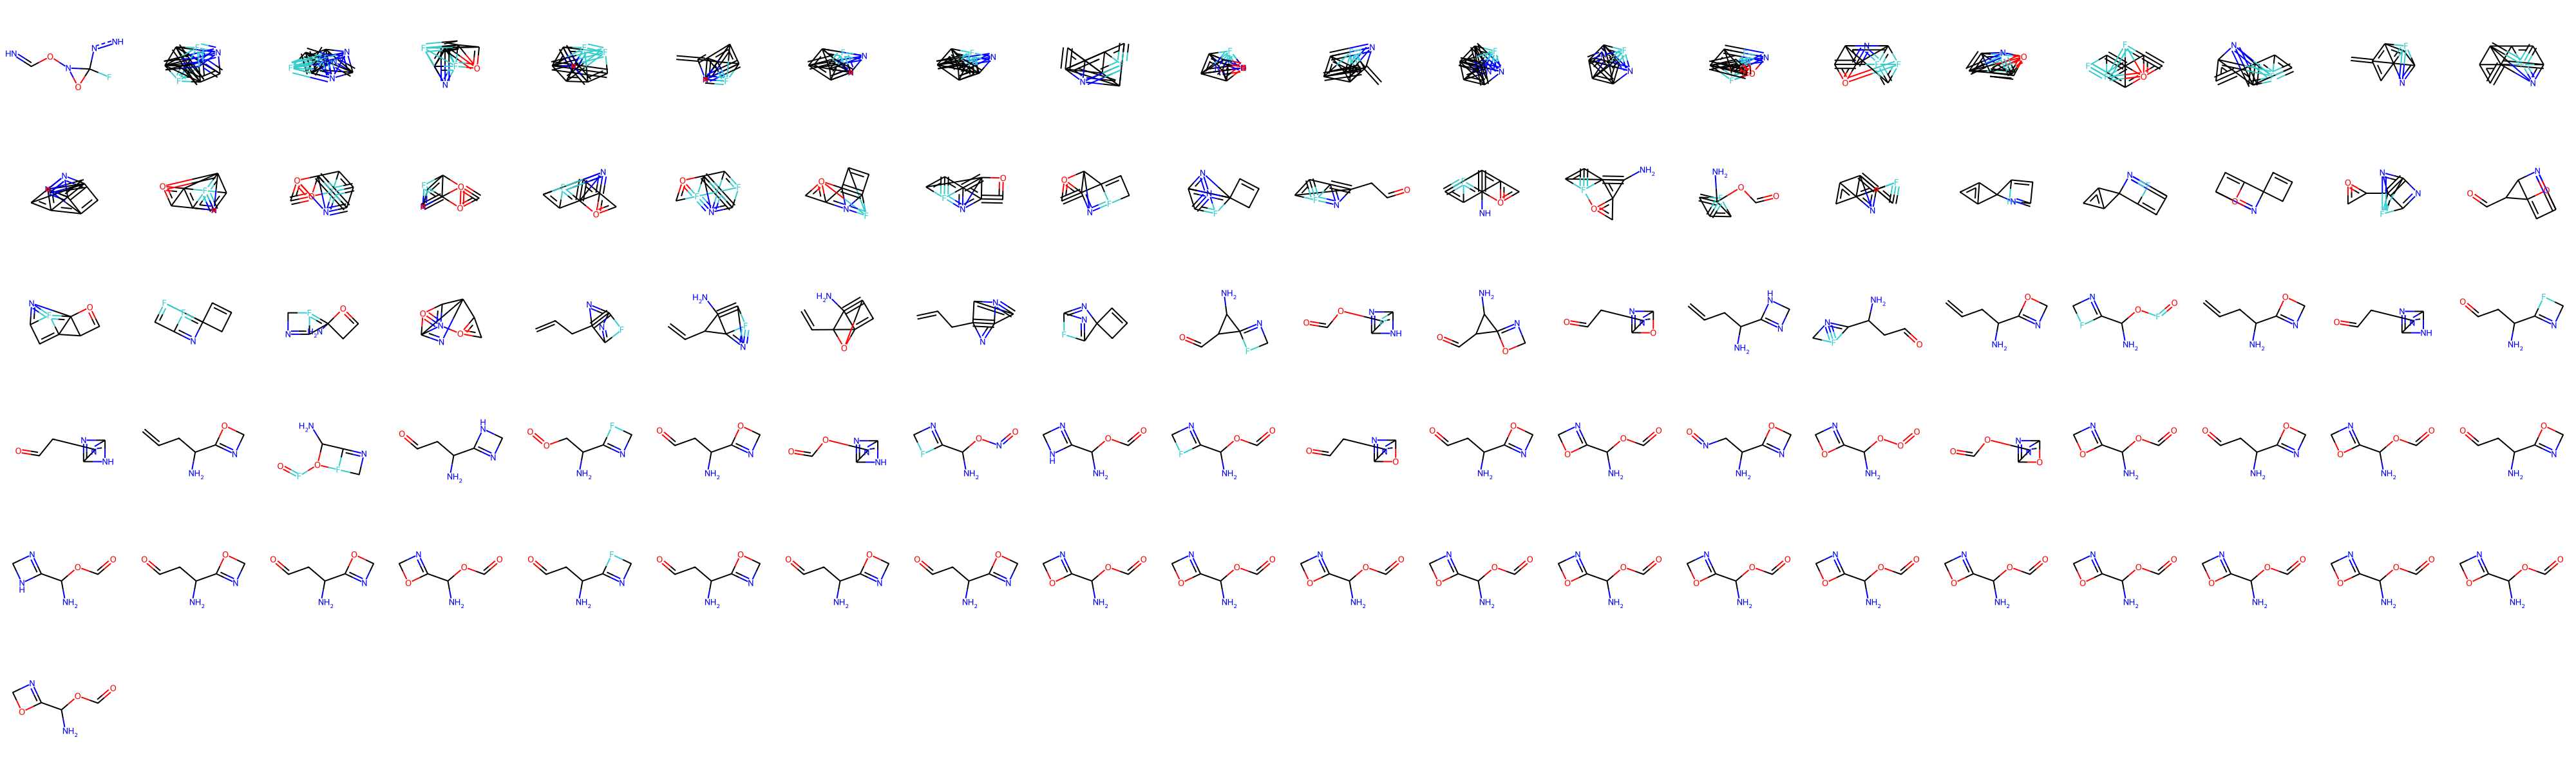
\includegraphics[width=\linewidth]{figures/multiprox/qm9_grid_image_single_noise.png}
    \caption[Best chain of molecule graphs obtained with MultiProx.]{Best chain of molecule graphs obtained with MultiProx and a ConGress denoiser. For this QM9 chain $n=10$, $m=100$, $t=50$ (10\% of $T$).
    }
    \label{fig:multiprox_qm9}
\end{figure}

From the figure, we can immediately discern issues not present in the image experiments. Namely, the warm-up phase for the molecules seems to last longer, and when it passes, the Gibbs chain seems to suffer from mode collapse relatively quickly.

Thus, when evaluating our MultiProx sampler on these discrete distributions, we observed that results could be greatly improved when adding in annealing steps before outputting the final graphs, i.e., employing the more general MultiProxAn sampler instead. The choice of moving the chain at a higher noise level $t$, then annealing to lower and lower $t'$ is empirically validated, as e.g., from Table~\ref{tab:qm9_stats} one observes that this always results in more valid molecules, but nevertheless always with less compute cost when compared to the baseline. As shown by Figure~\ref{fig:qm9_better}, the improvement in sample quality is also visually discernible. 

For an explanation, we hypothesize that the issue arises from the argmax projection of the Gaussian logits, which would require different guarantees on the modeling accuracy of its distribution. The higher noise level moves the Gibbs chain with a sufficiently high velocity so as to cover more modes, while the annealing steps to the lower noise level make sure there are fewer warm-up steps. We refer to the work by~\cite{sahoo_diffusion_2025} for a potential solution on how to remain in the single-noise-level configuration even for complex discrete distributions. 

\begin{table}[H]
    \centering
    \caption[MultiProxAn sampling metrics for the QM9 dataset of molecule graphs.]{Sampling metrics for each noise level hyperparameter configuration we tested for the QM9 dataset of molecule graphs. Left to right: MultiProxAn fixed noise level $t$ and final output noise level $t' \leq t$ (as percentages of $T$), percentage of valid molecule graphs, percentage of unique valid molecules, percentage of novel unique valid molecules (not present in the dataset), and total execution time of sampling. Arrows indicate whether higher or lower values of a metric are better. Best values per metric are in bold, while second-best values are underlined.}
    % \resizebox{\textwidth}{!}{
    \begin{tabular}{llrrrr}
        \toprule
         $t$ & $t'$ & $\uparrow$ Valid [\%] & $\uparrow$ Unique [\%] & $\uparrow$ Novel [\%] & $\downarrow$ Wall time [s]  \\
         \midrule
         \multicolumn{2}{l}{Baseline} & \underline{96.52} & 78.34 & 54.92 & 6302 \\
         50\% & 50\% & 0.00 & 0.00 & 0.00 & \textbf{151} \\
         50\% & 25\% & 0.16 & \textbf{100.0} & \textbf{96.01} & 1655 \\
         50\% & 10\% & 74.61 & 87.74 & 66.28 & 2561 \\
         50\% & 0.4\% & \textbf{96.62} & 77.95 & 55.20 & 3137 \\
         25\% & 25\% & 0.00 & 0.00 & 0.00 & \textbf{151} \\
         25\% & 10\% & 66.62 & \underline{90.35} & 70.49 & 1056 \\
         25\% & 0.4\% & 95.29 & 77.53 & 56.10 & 1418 \\
         10\% & 10\% & 14.52 & 30.64 & \underline{95.32} & \textbf{151} \\
         10\% & 0.4\% & 64.70 & 43.38 & 85.29 & \underline{513} \\
         \bottomrule
    \end{tabular}
    % }
    \label{tab:qm9_stats}
\end{table}

\begin{figure}[H]
    \centering
    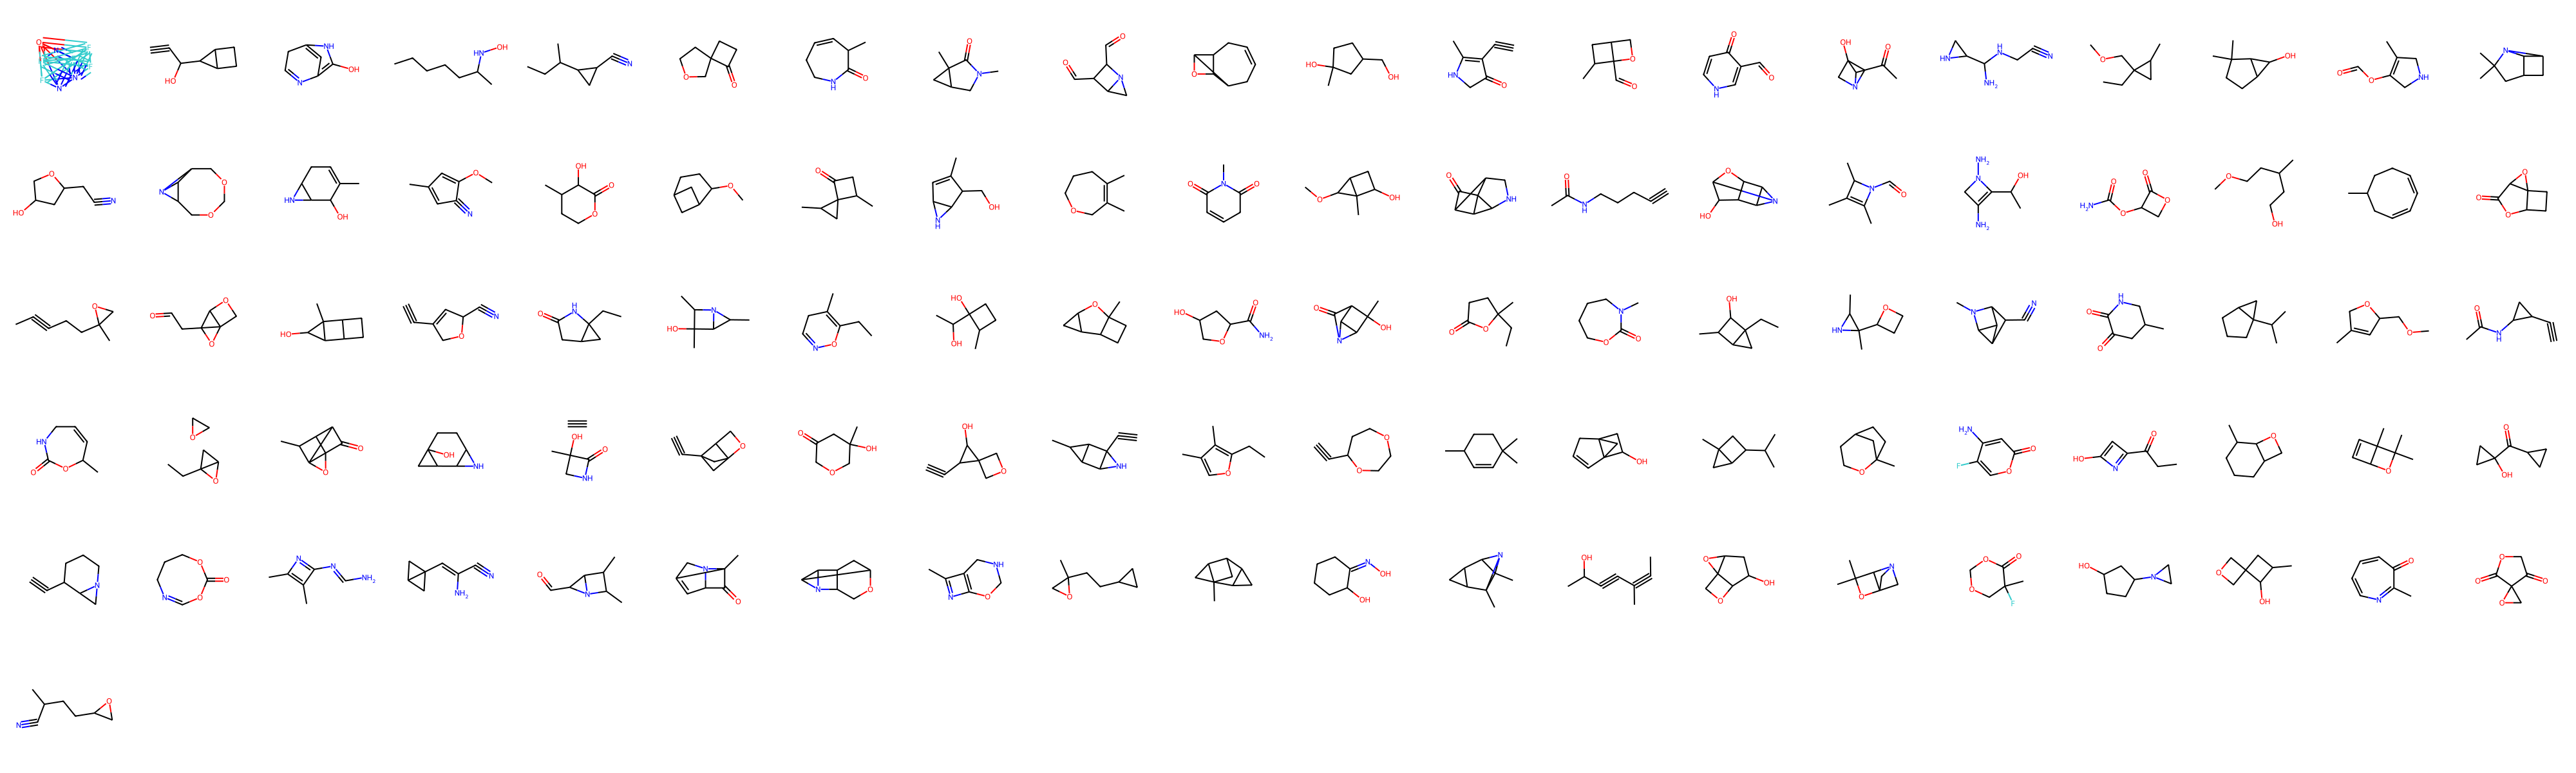
\includegraphics[width=\linewidth]{figures/multiprox/qm9_grid_image.png}
    \caption[Best chain of molecule graphs obtained with MultiProxAn.]{Best chain of molecule graphs obtained with MultiProxAn and a ConGress denoiser. For this QM9 chain $n=10$, $m=100$, $t=250$ and $t'=2$ (50\% and 0.4\% of $T$, respectively).
    }
    \label{fig:qm9_better}
\end{figure}

\subsection{Summary}

To conclude, we showed how by applying multimeasurement theory to denoising diffusion samplers, we can reproduce state-of-the-art performance metrics with much fewer denoising steps. Specifically, our MultiProxAn sampler can yield a speed-up factor of around $\frac{T}{t-t'+1}$ if we accept an increase in memory complexity by a factor of $m$, but experiments have shown that the values of the two fixed noise levels $t$ and $t'$ must be carefully validated. 

We again rise above purely reductionist and holistic approaches by taking a bit of each, this time to provide the best methods for sampling from multimodal distributions. We mix annealing approaches that assume it is enough to model noise step-by-step, and multimeasurement results that predict all relevant information lies in a single noise level. 